\part{Command line editing}
\begin{frame}
\partpage
\end{frame}

\section{Command Line Editing}
\begin{frame}{Section 6: Command line editing}
\begin{itemize}
\item Often you'll type a command or want to re-type a command
\item You can use keyboard shortcuts to find previously typed commands
\item The history and ctr + r are very useful
\end{itemize}
\end{frame}

\section{Finding Text}
\begin{frame}{Section 6: Grep}
\begin{itemize}
\item Often you'll want to search text files
\item grep is a powerful tool and can be used to find words or strings
\item Advanced users learn tools such as sed and awk to manipulate text
\item sed and awk are worth learning once you advance to shell scripting
\item sed -ie 's/annote/note/g' Dissertation-2-script.bib
\item Changes the word annote to note....
\end{itemize}
\end{frame}

\section{The Date}
\begin{frame}{Section 6: The Date}
\begin{itemize}
\item The date command lets you manipulate the format of the date
\item It becomes useful when you start writing scripts
\end{itemize}
\end{frame}

\section{The date in a script}
\begin{frame}{Section 6: The Date in a script}
\begin{figure}[h]
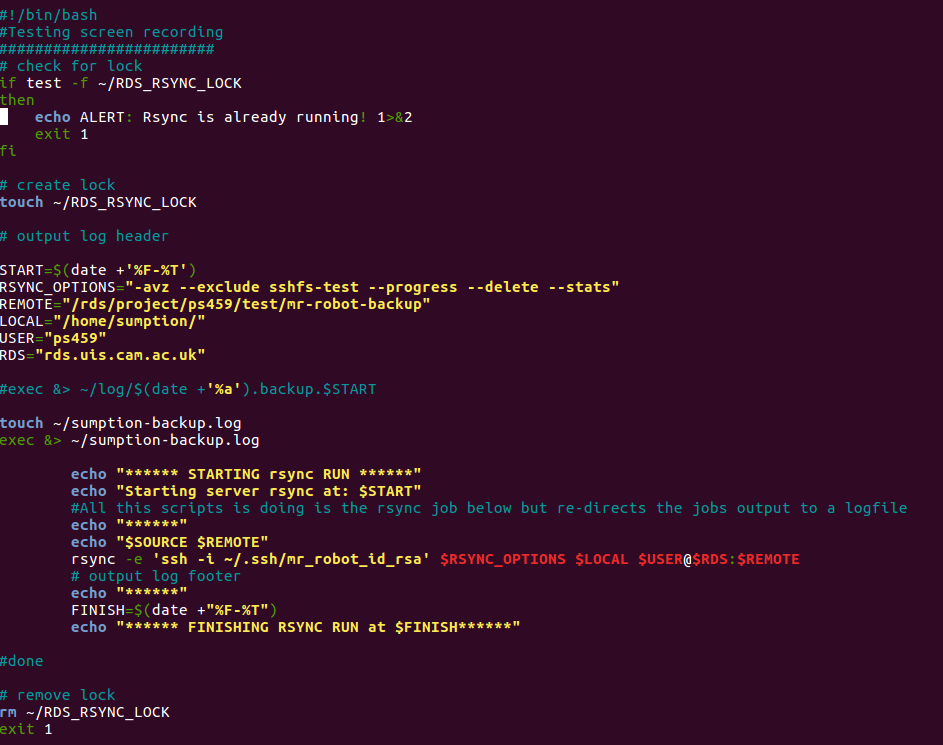
\includegraphics[height=0.8\textheight]{imgs/script-date.png}
\end{figure}
\end{frame}

\section{Exercises}
\begin{frame}{Section 6: Exercises}
\begin{itemize}
\item In the notes go to {Section 6: Command line editing}
\item Read the notes for Section 6 
\item Attempt exercises 14 to 16
\item Raise your hand if you are stuck
\item We can demonstrate or explain an exercise
\end{itemize}
\end{frame}

